\documentclass[1p]{elsarticle_modified}
%\bibliographystyle{elsarticle-num}

%\usepackage[colorlinks]{hyperref}
%\usepackage{abbrmath_seonhwa} %\Abb, \Ascr, \Acal ,\Abf, \Afrak
\usepackage{amsfonts}
\usepackage{amssymb}
\usepackage{amsmath}
\usepackage{amsthm}
\usepackage{scalefnt}
\usepackage{amsbsy}
\usepackage{kotex}
\usepackage{caption}
\usepackage{subfig}
\usepackage{color}
\usepackage{graphicx}
\usepackage{xcolor} %% white, black, red, green, blue, cyan, magenta, yellow
\usepackage{float}
\usepackage{setspace}
\usepackage{hyperref}

\usepackage{tikz}
\usetikzlibrary{arrows}

\usepackage{multirow}
\usepackage{array} % fixed length table
\usepackage{hhline}

%%%%%%%%%%%%%%%%%%%%%
\makeatletter
\renewcommand*\env@matrix[1][\arraystretch]{%
	\edef\arraystretch{#1}%
	\hskip -\arraycolsep
	\let\@ifnextchar\new@ifnextchar
	\array{*\c@MaxMatrixCols c}}
\makeatother %https://tex.stackexchange.com/questions/14071/how-can-i-increase-the-line-spacing-in-a-matrix
%%%%%%%%%%%%%%%

\usepackage[normalem]{ulem}

\newcommand{\msout}[1]{\ifmmode\text{\sout{\ensuremath{#1}}}\else\sout{#1}\fi}
%SOURCE: \msout is \stkout macro in https://tex.stackexchange.com/questions/20609/strikeout-in-math-mode

\newcommand{\cancel}[1]{
	\ifmmode
	{\color{red}\msout{#1}}
	\else
	{\color{red}\sout{#1}}
	\fi
}

\newcommand{\add}[1]{
	{\color{blue}\uwave{#1}}
}

\newcommand{\replace}[2]{
	\ifmmode
	{\color{red}\msout{#1}}{\color{blue}\uwave{#2}}
	\else
	{\color{red}\sout{#1}}{\color{blue}\uwave{#2}}
	\fi
}

\newcommand{\Sol}{\mathcal{S}} %segment
\newcommand{\D}{D} %diagram
\newcommand{\A}{\mathcal{A}} %arc


%%%%%%%%%%%%%%%%%%%%%%%%%%%%%5 test

\def\sl{\operatorname{\textup{SL}}(2,\Cbb)}
\def\psl{\operatorname{\textup{PSL}}(2,\Cbb)}
\def\quan{\mkern 1mu \triangleright \mkern 1mu}

\theoremstyle{definition}
\newtheorem{thm}{Theorem}[section]
\newtheorem{prop}[thm]{Proposition}
\newtheorem{lem}[thm]{Lemma}
\newtheorem{ques}[thm]{Question}
\newtheorem{cor}[thm]{Corollary}
\newtheorem{defn}[thm]{Definition}
\newtheorem{exam}[thm]{Example}
\newtheorem{rmk}[thm]{Remark}
\newtheorem{alg}[thm]{Algorithm}

\newcommand{\I}{\sqrt{-1}}
\begin{document}

%\begin{frontmatter}
%
%\title{Boundary parabolic representations of knots up to 8 crossings}
%
%%% Group authors per affiliation:
%\author{Yunhi Cho} 
%\address{Department of Mathematics, University of Seoul, Seoul, Korea}
%\ead{yhcho@uos.ac.kr}
%
%
%\author{Seonhwa Kim} %\fnref{s_kim}}
%\address{Center for Geometry and Physics, Institute for Basic Science, Pohang, 37673, Korea}
%\ead{ryeona17@ibs.re.kr}
%
%\author{Hyuk Kim}
%\address{Department of Mathematical Sciences, Seoul National University, Seoul 08826, Korea}
%\ead{hyukkim@snu.ac.kr}
%
%\author{Seokbeom Yoon}
%\address{Department of Mathematical Sciences, Seoul National University, Seoul, 08826,  Korea}
%\ead{sbyoon15@snu.ac.kr}
%
%\begin{abstract}
%We find all boundary parabolic representation of knots up to 8 crossings.
%
%\end{abstract}
%\begin{keyword}
%    \MSC[2010] 57M25 
%\end{keyword}
%
%\end{frontmatter}

%\linenumbers
%\tableofcontents
%
\newcommand\colored[1]{\textcolor{white}{\rule[-0.35ex]{0.8em}{1.4ex}}\kern-0.8em\color{red} #1}%
%\newcommand\colored[1]{\textcolor{white}{ #1}\kern-2.17ex	\textcolor{white}{ #1}\kern-1.81ex	\textcolor{white}{ #1}\kern-2.15ex\color{red}#1	}

{\Large $\underline{12n_{0037}~(K12n_{0037})}$}

\setlength{\tabcolsep}{10pt}
\renewcommand{\arraystretch}{1.6}
\vspace{1cm}\begin{tabular}{m{100pt}>{\centering\arraybackslash}m{274pt}}
\multirow{5}{120pt}{
	\centering
	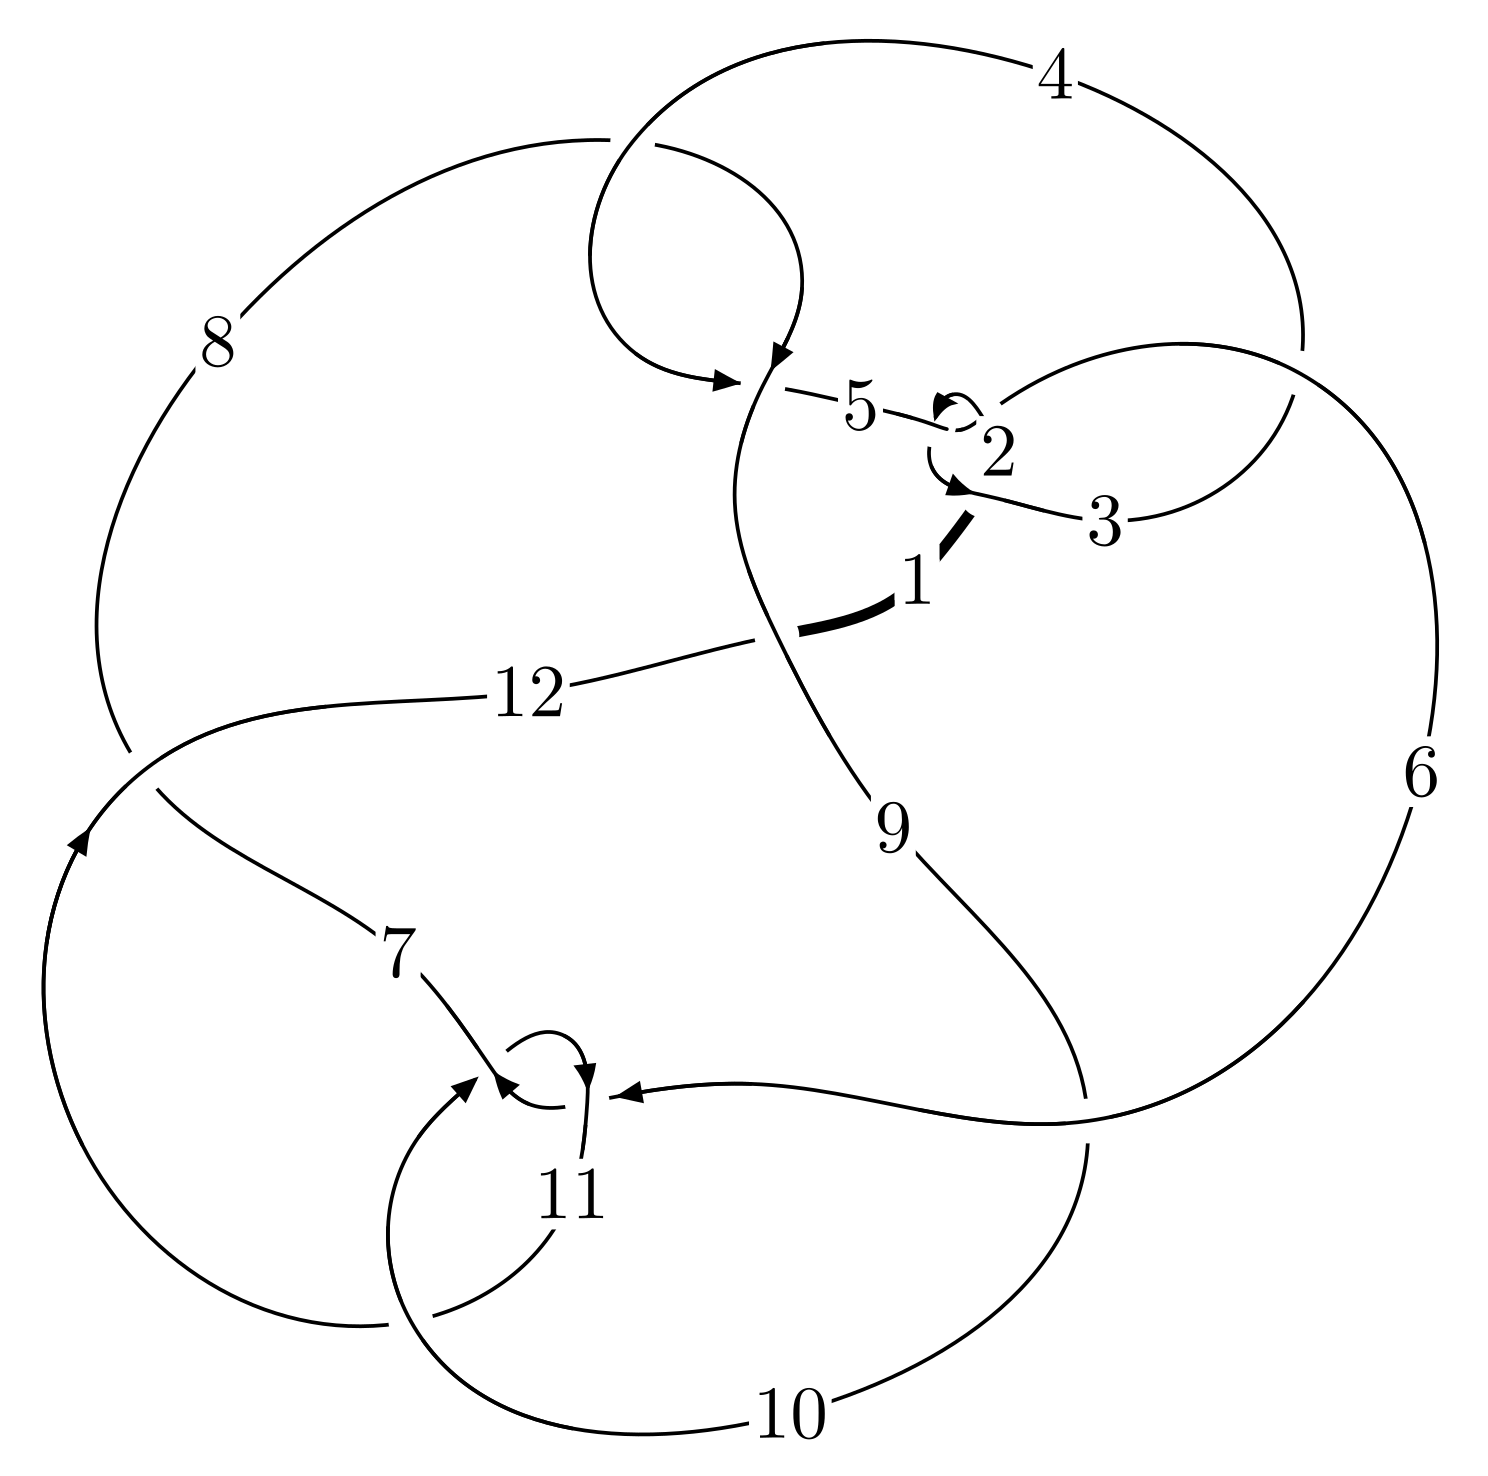
\includegraphics[width=112pt]{../../../GIT/diagram.site/Diagrams/png/2126_12n_0037.png}\\
\ \ \ A knot diagram\footnotemark}&
\allowdisplaybreaks
\textbf{Linearized knot diagam} \\
\cline{2-2}
 &
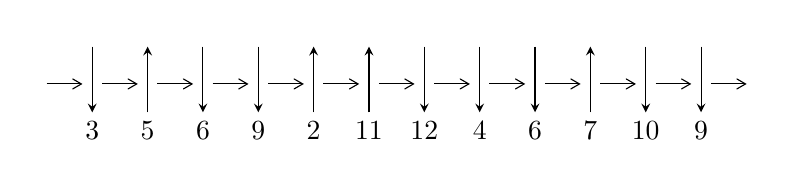
\begin{tikzpicture}[x=20pt, y=17pt]
	% nodes
	\node (C0) at (0, 0) {};
	\node (C1) at (1, 0) {};
	\node (C1U) at (1, +1) {};
	\node (C1D) at (1, -1) {3};

	\node (C2) at (2, 0) {};
	\node (C2U) at (2, +1) {};
	\node (C2D) at (2, -1) {5};

	\node (C3) at (3, 0) {};
	\node (C3U) at (3, +1) {};
	\node (C3D) at (3, -1) {6};

	\node (C4) at (4, 0) {};
	\node (C4U) at (4, +1) {};
	\node (C4D) at (4, -1) {9};

	\node (C5) at (5, 0) {};
	\node (C5U) at (5, +1) {};
	\node (C5D) at (5, -1) {2};

	\node (C6) at (6, 0) {};
	\node (C6U) at (6, +1) {};
	\node (C6D) at (6, -1) {11};

	\node (C7) at (7, 0) {};
	\node (C7U) at (7, +1) {};
	\node (C7D) at (7, -1) {12};

	\node (C8) at (8, 0) {};
	\node (C8U) at (8, +1) {};
	\node (C8D) at (8, -1) {4};

	\node (C9) at (9, 0) {};
	\node (C9U) at (9, +1) {};
	\node (C9D) at (9, -1) {6};

	\node (C10) at (10, 0) {};
	\node (C10U) at (10, +1) {};
	\node (C10D) at (10, -1) {7};

	\node (C11) at (11, 0) {};
	\node (C11U) at (11, +1) {};
	\node (C11D) at (11, -1) {10};

	\node (C12) at (12, 0) {};
	\node (C12U) at (12, +1) {};
	\node (C12D) at (12, -1) {9};
	\node (C13) at (13, 0) {};

	% arrows
	\draw[->,>={angle 60}]
	(C0) edge (C1) (C1) edge (C2) (C2) edge (C3) (C3) edge (C4) (C4) edge (C5) (C5) edge (C6) (C6) edge (C7) (C7) edge (C8) (C8) edge (C9) (C9) edge (C10) (C10) edge (C11) (C11) edge (C12) (C12) edge (C13) ;	\draw[->,>=stealth]
	(C1U) edge (C1D) (C2D) edge (C2U) (C3U) edge (C3D) (C4U) edge (C4D) (C5D) edge (C5U) (C6D) edge (C6U) (C7U) edge (C7D) (C8U) edge (C8D) (C9U) edge (C9D) (C10D) edge (C10U) (C11U) edge (C11D) (C12U) edge (C12D) ;
	\end{tikzpicture} \\
\hhline{~~} \\& 
\textbf{Solving Sequence} \\ \cline{2-2} 
 &
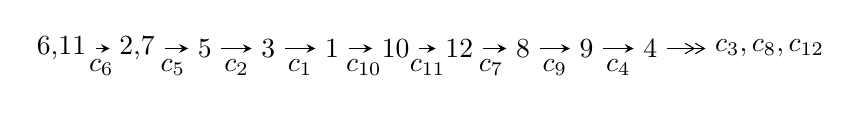
\begin{tikzpicture}[x=23pt, y=7pt]
	% node
	\node (A0) at (-1/8, 0) {6,11};
	\node (A1) at (17/16, 0) {2,7};
	\node (A2) at (17/8, 0) {5};
	\node (A3) at (25/8, 0) {3};
	\node (A4) at (33/8, 0) {1};
	\node (A5) at (41/8, 0) {10};
	\node (A6) at (49/8, 0) {12};
	\node (A7) at (57/8, 0) {8};
	\node (A8) at (65/8, 0) {9};
	\node (A9) at (73/8, 0) {4};
	\node (C1) at (1/2, -1) {$c_{6}$};
	\node (C2) at (13/8, -1) {$c_{5}$};
	\node (C3) at (21/8, -1) {$c_{2}$};
	\node (C4) at (29/8, -1) {$c_{1}$};
	\node (C5) at (37/8, -1) {$c_{10}$};
	\node (C6) at (45/8, -1) {$c_{11}$};
	\node (C7) at (53/8, -1) {$c_{7}$};
	\node (C8) at (61/8, -1) {$c_{9}$};
	\node (C9) at (69/8, -1) {$c_{4}$};
	\node (A10) at (11, 0) {$c_{3},c_{8},c_{12}$};

	% edge
	\draw[->,>=stealth]	
	(A0) edge (A1) (A1) edge (A2) (A2) edge (A3) (A3) edge (A4) (A4) edge (A5) (A5) edge (A6) (A6) edge (A7) (A7) edge (A8) (A8) edge (A9) ;
	\draw[->>,>={angle 60}]	
	(A9) edge (A10);
\end{tikzpicture} \\ 

\end{tabular} \\

\footnotetext{
The image of knot diagram is generated by the software ``\textbf{Draw programme}" developed by Andrew Bartholomew(\url{http://www.layer8.co.uk/maths/draw/index.htm\#Running-draw}), where we modified some parts for our purpose(\url{https://github.com/CATsTAILs/LinksPainter}).
}\phantom \\ \newline 
\centering \textbf{Ideals for irreducible components\footnotemark of $X_{\text{par}}$} 
 
\begin{align*}
I^u_{1}&=\langle 
u^{28}-2 u^{27}+\cdots+2 b-3 u,\;2 u^{28}-4 u^{27}+\cdots+2 a-2,\;u^{30}-3 u^{29}+\cdots+4 u-1\rangle \\
I^u_{2}&=\langle 
-2 u^4 a-4 u^3 a-2 u^4+3 u^2 a-4 u^3-8 a u+3 u^2+19 b-7 a-8 u-7,\\
\phantom{I^u_{2}}&\phantom{= \langle  }u^3 a- u^2 a-2 u^3+a^2+a u+2 u^2- u+2,\;u^5- u^4+2 u^3- u^2+u-1\rangle \\
\\
\end{align*}
\raggedright * 2 irreducible components of $\dim_{\mathbb{C}}=0$, with total 40 representations.\\
\footnotetext{All coefficients of polynomials are rational numbers. But the coefficients are sometimes approximated in decimal forms when there is not enough margin.}
\newpage
\renewcommand{\arraystretch}{1}
\centering \section*{I. $I^u_{1}= \langle u^{28}-2 u^{27}+\cdots+2 b-3 u,\;2 u^{28}-4 u^{27}+\cdots+2 a-2,\;u^{30}-3 u^{29}+\cdots+4 u-1 \rangle$}
\flushleft \textbf{(i) Arc colorings}\\
\begin{tabular}{m{7pt} m{180pt} m{7pt} m{180pt} }
\flushright $a_{6}=$&$\begin{pmatrix}1\\0\end{pmatrix}$ \\
\flushright $a_{11}=$&$\begin{pmatrix}0\\u\end{pmatrix}$ \\
\flushright $a_{2}=$&$\begin{pmatrix}- u^{28}+2 u^{27}+\cdots+\frac{3}{2} u+1\\-\frac{1}{2} u^{28}+u^{27}+\cdots+\frac{5}{2} u^2+\frac{3}{2} u\end{pmatrix}$ \\
\flushright $a_{7}=$&$\begin{pmatrix}1\\- u^2\end{pmatrix}$ \\
\flushright $a_{5}=$&$\begin{pmatrix}-\frac{1}{2} u^{28}+2 u^{27}+\cdots+\frac{3}{2} u^3+4 u\\-\frac{1}{2} u^{28}+2 u^{27}+\cdots+\frac{17}{2} u^2-\frac{3}{2} u\end{pmatrix}$ \\
\flushright $a_{3}=$&$\begin{pmatrix}-3 u^{28}+6 u^{27}+\cdots+\frac{17}{2} u^2+\frac{5}{2} u\\-\frac{3}{2} u^{28}+3 u^{27}+\cdots+\frac{17}{2} u^2-\frac{3}{2} u\end{pmatrix}$ \\
\flushright $a_{1}=$&$\begin{pmatrix}- u^{11}-2 u^9-2 u^7- u^3\\- u^{11}-3 u^9-4 u^7- u^5+u^3+u\end{pmatrix}$ \\
\flushright $a_{10}=$&$\begin{pmatrix}- u\\u^3+u\end{pmatrix}$ \\
\flushright $a_{12}=$&$\begin{pmatrix}- u^3\\u^5+u^3+u\end{pmatrix}$ \\
\flushright $a_{8}=$&$\begin{pmatrix}- u^6- u^4+1\\u^8+2 u^6+2 u^4\end{pmatrix}$ \\
\flushright $a_{9}=$&$\begin{pmatrix}u^3\\u^3+u\end{pmatrix}$ \\
\flushright $a_{4}=$&$\begin{pmatrix}-\frac{3}{2} u^{28}+3 u^{27}+\cdots+\frac{3}{2} u^3+4 u\\-\frac{3}{2} u^{28}+3 u^{27}+\cdots+\frac{17}{2} u^2-\frac{3}{2} u\end{pmatrix}$\\&\end{tabular}
\flushleft \textbf{(ii) Obstruction class $= -1$}\\~\\
\flushleft \textbf{(iii) Cusp Shapes $= 4 u^{29}-\frac{25}{2} u^{28}+\cdots-\frac{59}{2} u+\frac{7}{2}$}\\~\\
\newpage\renewcommand{\arraystretch}{1}
\flushleft \textbf{(iv) u-Polynomials at the component}\newline \\
\begin{tabular}{m{50pt}|m{274pt}}
Crossings & \hspace{64pt}u-Polynomials at each crossing \\
\hline $$\begin{aligned}c_{1}\end{aligned}$$&$\begin{aligned}
&u^{30}+22 u^{29}+\cdots+23 u+1
\end{aligned}$\\
\hline $$\begin{aligned}c_{2},c_{5}\end{aligned}$$&$\begin{aligned}
&u^{30}+6 u^{29}+\cdots+5 u+1
\end{aligned}$\\
\hline $$\begin{aligned}c_{3}\end{aligned}$$&$\begin{aligned}
&u^{30}-6 u^{29}+\cdots+5 u+1
\end{aligned}$\\
\hline $$\begin{aligned}c_{4},c_{8}\end{aligned}$$&$\begin{aligned}
&u^{30}- u^{29}+\cdots-2048 u-1024
\end{aligned}$\\
\hline $$\begin{aligned}c_{6},c_{10}\end{aligned}$$&$\begin{aligned}
&u^{30}-3 u^{29}+\cdots+4 u-1
\end{aligned}$\\
\hline $$\begin{aligned}c_{7},c_{9}\end{aligned}$$&$\begin{aligned}
&u^{30}+3 u^{29}+\cdots+2 u-1
\end{aligned}$\\
\hline $$\begin{aligned}c_{11}\end{aligned}$$&$\begin{aligned}
&u^{30}+19 u^{29}+\cdots+8 u+1
\end{aligned}$\\
\hline $$\begin{aligned}c_{12}\end{aligned}$$&$\begin{aligned}
&u^{30}-13 u^{29}+\cdots-29592 u+1669
\end{aligned}$\\
\hline
\end{tabular}\\~\\
\newpage\renewcommand{\arraystretch}{1}
\flushleft \textbf{(v) Riley Polynomials at the component}\newline \\
\begin{tabular}{m{50pt}|m{274pt}}
Crossings & \hspace{64pt}Riley Polynomials at each crossing \\
\hline $$\begin{aligned}c_{1}\end{aligned}$$&$\begin{aligned}
&y^{30}-22 y^{29}+\cdots-241 y+1
\end{aligned}$\\
\hline $$\begin{aligned}c_{2},c_{5}\end{aligned}$$&$\begin{aligned}
&y^{30}+22 y^{29}+\cdots+23 y+1
\end{aligned}$\\
\hline $$\begin{aligned}c_{3}\end{aligned}$$&$\begin{aligned}
&y^{30}-66 y^{29}+\cdots+199 y+1
\end{aligned}$\\
\hline $$\begin{aligned}c_{4},c_{8}\end{aligned}$$&$\begin{aligned}
&y^{30}-55 y^{29}+\cdots-4194304 y+1048576
\end{aligned}$\\
\hline $$\begin{aligned}c_{6},c_{10}\end{aligned}$$&$\begin{aligned}
&y^{30}+19 y^{29}+\cdots+8 y+1
\end{aligned}$\\
\hline $$\begin{aligned}c_{7},c_{9}\end{aligned}$$&$\begin{aligned}
&y^{30}-45 y^{29}+\cdots+8 y+1
\end{aligned}$\\
\hline $$\begin{aligned}c_{11}\end{aligned}$$&$\begin{aligned}
&y^{30}-13 y^{29}+\cdots+36 y+1
\end{aligned}$\\
\hline $$\begin{aligned}c_{12}\end{aligned}$$&$\begin{aligned}
&y^{30}-145 y^{29}+\cdots-1268048336 y+2785561
\end{aligned}$\\
\hline
\end{tabular}\\~\\
\newpage\flushleft \textbf{(vi) Complex Volumes and Cusp Shapes}
$$\begin{array}{c|c|c}  
\text{Solutions to }I^u_{1}& \I (\text{vol} + \sqrt{-1}CS) & \text{Cusp shape}\\
 \hline 
\begin{aligned}
u &= \phantom{-}0.976696 + 0.048976 I \\
a &= \phantom{-}0.12463 + 2.08766 I \\
b &= -0.56420 + 1.41173 I\end{aligned}
 & -16.9810 - 6.1121 I & -7.59589 + 2.67108 I \\ \hline\begin{aligned}
u &= \phantom{-}0.976696 - 0.048976 I \\
a &= \phantom{-}0.12463 - 2.08766 I \\
b &= -0.56420 - 1.41173 I\end{aligned}
 & -16.9810 + 6.1121 I & -7.59589 - 2.67108 I \\ \hline\begin{aligned}
u &= \phantom{-}0.465293 + 0.912238 I \\
a &= \phantom{-}1.93554 - 1.46111 I \\
b &= \phantom{-}0.008467 - 0.943478 I\end{aligned}
 & -1.62988 + 2.08354 I & -8.16060 - 3.45084 I \\ \hline\begin{aligned}
u &= \phantom{-}0.465293 - 0.912238 I \\
a &= \phantom{-}1.93554 + 1.46111 I \\
b &= \phantom{-}0.008467 + 0.943478 I\end{aligned}
 & -1.62988 - 2.08354 I & -8.16060 + 3.45084 I \\ \hline\begin{aligned}
u &= \phantom{-}0.960868\phantom{ +0.000000I} \\
a &= -0.707740\phantom{ +0.000000I} \\
b &= -1.15384\phantom{ +0.000000I}\end{aligned}
 & -12.5512\phantom{ +0.000000I} & -5.29830\phantom{ +0.000000I} \\ \hline\begin{aligned}
u &= -0.166593 + 0.933326 I \\
a &= -0.92254 - 2.23571 I \\
b &= \phantom{-}0.617718 - 0.920078 I\end{aligned}
 & -1.07529 - 3.17191 I & -11.28317 + 2.37568 I \\ \hline\begin{aligned}
u &= -0.166593 - 0.933326 I \\
a &= -0.92254 + 2.23571 I \\
b &= \phantom{-}0.617718 + 0.920078 I\end{aligned}
 & -1.07529 + 3.17191 I & -11.28317 - 2.37568 I \\ \hline\begin{aligned}
u &= \phantom{-}0.231283 + 1.116780 I \\
a &= -0.01646 + 3.64757 I \\
b &= \phantom{-}0.357122 + 1.153660 I\end{aligned}
 & -3.77750 + 3.57782 I & -10.98746 - 4.01828 I \\ \hline\begin{aligned}
u &= \phantom{-}0.231283 - 1.116780 I \\
a &= -0.01646 - 3.64757 I \\
b &= \phantom{-}0.357122 - 1.153660 I\end{aligned}
 & -3.77750 - 3.57782 I & -10.98746 + 4.01828 I \\ \hline\begin{aligned}
u &= -0.828254 + 0.182083 I \\
a &= \phantom{-}0.61725 - 1.74485 I \\
b &= -0.176405 - 1.246890 I\end{aligned}
 & -5.31113 + 2.21238 I & -8.26070 - 1.34538 I\\
 \hline 
 \end{array}$$\newpage$$\begin{array}{c|c|c}  
\text{Solutions to }I^u_{1}& \I (\text{vol} + \sqrt{-1}CS) & \text{Cusp shape}\\
 \hline 
\begin{aligned}
u &= -0.828254 - 0.182083 I \\
a &= \phantom{-}0.61725 + 1.74485 I \\
b &= -0.176405 + 1.246890 I\end{aligned}
 & -5.31113 - 2.21238 I & -8.26070 + 1.34538 I \\ \hline\begin{aligned}
u &= \phantom{-}0.247708 + 0.775830 I \\
a &= \phantom{-}0.759182 + 0.262675 I \\
b &= \phantom{-}0.064907 + 0.268421 I\end{aligned}
 & -0.445314 + 1.227680 I & -5.13147 - 5.35598 I \\ \hline\begin{aligned}
u &= \phantom{-}0.247708 - 0.775830 I \\
a &= \phantom{-}0.759182 - 0.262675 I \\
b &= \phantom{-}0.064907 - 0.268421 I\end{aligned}
 & -0.445314 - 1.227680 I & -5.13147 + 5.35598 I \\ \hline\begin{aligned}
u &= -0.431100 + 1.154270 I \\
a &= -0.376542 + 0.218469 I \\
b &= -0.568898 - 0.159015 I\end{aligned}
 & -4.80479 - 4.01525 I & -8.38777 + 4.38030 I \\ \hline\begin{aligned}
u &= -0.431100 - 1.154270 I \\
a &= -0.376542 - 0.218469 I \\
b &= -0.568898 + 0.159015 I\end{aligned}
 & -4.80479 + 4.01525 I & -8.38777 - 4.38030 I \\ \hline\begin{aligned}
u &= -0.538187 + 1.166640 I \\
a &= \phantom{-}1.43637 + 2.76799 I \\
b &= -0.271108 + 1.248230 I\end{aligned}
 & -8.20594 - 7.19126 I & -10.97609 + 5.35204 I \\ \hline\begin{aligned}
u &= -0.538187 - 1.166640 I \\
a &= \phantom{-}1.43637 - 2.76799 I \\
b &= -0.271108 - 1.248230 I\end{aligned}
 & -8.20594 + 7.19126 I & -10.97609 - 5.35204 I \\ \hline\begin{aligned}
u &= -0.033664 + 0.692526 I \\
a &= \phantom{-}1.161840 - 0.009465 I \\
b &= \phantom{-}0.453127 + 0.691055 I\end{aligned}
 & -0.304353 + 1.377760 I & -5.31625 - 4.96434 I \\ \hline\begin{aligned}
u &= -0.033664 - 0.692526 I \\
a &= \phantom{-}1.161840 + 0.009465 I \\
b &= \phantom{-}0.453127 - 0.691055 I\end{aligned}
 & -0.304353 - 1.377760 I & -5.31625 + 4.96434 I \\ \hline\begin{aligned}
u &= -0.343267 + 1.272440 I \\
a &= -0.45988 - 3.28730 I \\
b &= -0.116378 - 1.358180 I\end{aligned}
 & -9.80427 - 1.78849 I & -12.19268 + 1.56602 I\\
 \hline 
 \end{array}$$\newpage$$\begin{array}{c|c|c}  
\text{Solutions to }I^u_{1}& \I (\text{vol} + \sqrt{-1}CS) & \text{Cusp shape}\\
 \hline 
\begin{aligned}
u &= -0.343267 - 1.272440 I \\
a &= -0.45988 + 3.28730 I \\
b &= -0.116378 + 1.358180 I\end{aligned}
 & -9.80427 + 1.78849 I & -12.19268 - 1.56602 I \\ \hline\begin{aligned}
u &= -0.662170\phantom{ +0.000000I} \\
a &= \phantom{-}0.443818\phantom{ +0.000000I} \\
b &= -0.426253\phantom{ +0.000000I}\end{aligned}
 & -1.60545\phantom{ +0.000000I} & -5.56060\phantom{ +0.000000I} \\ \hline\begin{aligned}
u &= \phantom{-}0.486497 + 1.299810 I \\
a &= -1.68061 - 0.72887 I \\
b &= -1.177550 + 0.042833 I\end{aligned}
 & -16.5686 + 5.1451 I & -8.39302 - 2.77801 I \\ \hline\begin{aligned}
u &= \phantom{-}0.486497 - 1.299810 I \\
a &= -1.68061 + 0.72887 I \\
b &= -1.177550 - 0.042833 I\end{aligned}
 & -16.5686 - 5.1451 I & -8.39302 + 2.77801 I \\ \hline\begin{aligned}
u &= \phantom{-}0.517727 + 1.292950 I \\
a &= \phantom{-}0.64113 - 3.50293 I \\
b &= -0.59774 - 1.40210 I\end{aligned}
 & \phantom{-}18.6656 + 11.4427 I & -10.35634 - 5.55493 I \\ \hline\begin{aligned}
u &= \phantom{-}0.517727 - 1.292950 I \\
a &= \phantom{-}0.64113 + 3.50293 I \\
b &= -0.59774 + 1.40210 I\end{aligned}
 & \phantom{-}18.6656 - 11.4427 I & -10.35634 + 5.55493 I \\ \hline\begin{aligned}
u &= \phantom{-}0.459310 + 1.324670 I \\
a &= -1.26343 + 2.96678 I \\
b &= -0.55077 + 1.45009 I\end{aligned}
 & \phantom{-}18.1990 - 1.0261 I & -10.88309 + 0. I\phantom{ +0.000000I} \\ \hline\begin{aligned}
u &= \phantom{-}0.459310 - 1.324670 I \\
a &= -1.26343 - 2.96678 I \\
b &= -0.55077 - 1.45009 I\end{aligned}
 & \phantom{-}18.1990 + 1.0261 I & -10.88309 + 0. I\phantom{ +0.000000I} \\ \hline\begin{aligned}
u &= \phantom{-}0.307204 + 0.297461 I \\
a &= \phantom{-}1.17548 + 0.93277 I \\
b &= \phantom{-}0.311753 + 0.846408 I\end{aligned}
 & -0.35666 + 1.51654 I & -2.64602 - 3.80074 I \\ \hline\begin{aligned}
u &= \phantom{-}0.307204 - 0.297461 I \\
a &= \phantom{-}1.17548 - 0.93277 I \\
b &= \phantom{-}0.311753 - 0.846408 I\end{aligned}
 & -0.35666 - 1.51654 I & -2.64602 + 3.80074 I\\
 \hline 
 \end{array}$$\newpage\newpage\renewcommand{\arraystretch}{1}
\centering \section*{II. $I^u_{2}= \langle -2 u^4 a-2 u^4+\cdots-7 a-7,\;u^3 a- u^2 a-2 u^3+a^2+a u+2 u^2- u+2,\;u^5- u^4+2 u^3- u^2+u-1 \rangle$}
\flushleft \textbf{(i) Arc colorings}\\
\begin{tabular}{m{7pt} m{180pt} m{7pt} m{180pt} }
\flushright $a_{6}=$&$\begin{pmatrix}1\\0\end{pmatrix}$ \\
\flushright $a_{11}=$&$\begin{pmatrix}0\\u\end{pmatrix}$ \\
\flushright $a_{2}=$&$\begin{pmatrix}a\\0.105263 a u^{4}+0.105263 u^{4}+\cdots+0.368421 a+0.368421\end{pmatrix}$ \\
\flushright $a_{7}=$&$\begin{pmatrix}1\\- u^2\end{pmatrix}$ \\
\flushright $a_{5}=$&$\begin{pmatrix}-0.105263 a u^{4}-0.105263 u^{4}+\cdots+0.631579 a-0.368421\\0.105263 a u^{4}+0.105263 u^{4}+\cdots+0.368421 a-0.631579\end{pmatrix}$ \\
\flushright $a_{3}=$&$\begin{pmatrix}u^3- u^2+a+u-1\\0.105263 a u^{4}+0.105263 u^{4}+\cdots+0.368421 a-0.631579\end{pmatrix}$ \\
\flushright $a_{1}=$&$\begin{pmatrix}-1\\0\end{pmatrix}$ \\
\flushright $a_{10}=$&$\begin{pmatrix}- u\\u^3+u\end{pmatrix}$ \\
\flushright $a_{12}=$&$\begin{pmatrix}- u^3\\u^4- u^3+u^2+1\end{pmatrix}$ \\
\flushright $a_{8}=$&$\begin{pmatrix}u^3\\u^3+u\end{pmatrix}$ \\
\flushright $a_{9}=$&$\begin{pmatrix}u^3\\u^3+u\end{pmatrix}$ \\
\flushright $a_{4}=$&$\begin{pmatrix}-0.105263 a u^{4}-0.105263 u^{4}+\cdots+0.631579 a-0.368421\\0.105263 a u^{4}+0.105263 u^{4}+\cdots+0.368421 a-0.631579\end{pmatrix}$\\&\end{tabular}
\flushleft \textbf{(ii) Obstruction class $= 1$}\\~\\
\flushleft \textbf{(iii) Cusp Shapes $= \frac{3}{19} u^4 a-\frac{13}{19} u^3 a-\frac{16}{19} u^4+\frac{5}{19} u^2 a+\frac{82}{19} u^3-\frac{7}{19} a u-\frac{90}{19} u^2-\frac{37}{19} a+\frac{69}{19} u-\frac{170}{19}$}\\~\\
\newpage\renewcommand{\arraystretch}{1}
\flushleft \textbf{(iv) u-Polynomials at the component}\newline \\
\begin{tabular}{m{50pt}|m{274pt}}
Crossings & \hspace{64pt}u-Polynomials at each crossing \\
\hline $$\begin{aligned}c_{1},c_{3},c_{5}\end{aligned}$$&$\begin{aligned}
&(u^2- u+1)^5
\end{aligned}$\\
\hline $$\begin{aligned}c_{2}\end{aligned}$$&$\begin{aligned}
&(u^2+u+1)^5
\end{aligned}$\\
\hline $$\begin{aligned}c_{4},c_{8}\end{aligned}$$&$\begin{aligned}
&u^{10}
\end{aligned}$\\
\hline $$\begin{aligned}c_{6}\end{aligned}$$&$\begin{aligned}
&(u^5- u^4+2 u^3- u^2+u-1)^2
\end{aligned}$\\
\hline $$\begin{aligned}c_{7}\end{aligned}$$&$\begin{aligned}
&(u^5+u^4-2 u^3- u^2+u-1)^2
\end{aligned}$\\
\hline $$\begin{aligned}c_{9},c_{12}\end{aligned}$$&$\begin{aligned}
&(u^5- u^4-2 u^3+u^2+u+1)^2
\end{aligned}$\\
\hline $$\begin{aligned}c_{10}\end{aligned}$$&$\begin{aligned}
&(u^5+u^4+2 u^3+u^2+u+1)^2
\end{aligned}$\\
\hline $$\begin{aligned}c_{11}\end{aligned}$$&$\begin{aligned}
&(u^5+3 u^4+4 u^3+u^2- u-1)^2
\end{aligned}$\\
\hline
\end{tabular}\\~\\
\newpage\renewcommand{\arraystretch}{1}
\flushleft \textbf{(v) Riley Polynomials at the component}\newline \\
\begin{tabular}{m{50pt}|m{274pt}}
Crossings & \hspace{64pt}Riley Polynomials at each crossing \\
\hline $$\begin{aligned}c_{1},c_{2},c_{3}\\c_{5}\end{aligned}$$&$\begin{aligned}
&(y^2+y+1)^5
\end{aligned}$\\
\hline $$\begin{aligned}c_{4},c_{8}\end{aligned}$$&$\begin{aligned}
&y^{10}
\end{aligned}$\\
\hline $$\begin{aligned}c_{6},c_{10}\end{aligned}$$&$\begin{aligned}
&(y^5+3 y^4+4 y^3+y^2- y-1)^2
\end{aligned}$\\
\hline $$\begin{aligned}c_{7},c_{9},c_{12}\end{aligned}$$&$\begin{aligned}
&(y^5-5 y^4+8 y^3-3 y^2- y-1)^2
\end{aligned}$\\
\hline $$\begin{aligned}c_{11}\end{aligned}$$&$\begin{aligned}
&(y^5- y^4+8 y^3-3 y^2+3 y-1)^2
\end{aligned}$\\
\hline
\end{tabular}\\~\\
\newpage\flushleft \textbf{(vi) Complex Volumes and Cusp Shapes}
$$\begin{array}{c|c|c}  
\text{Solutions to }I^u_{2}& \I (\text{vol} + \sqrt{-1}CS) & \text{Cusp shape}\\
 \hline 
\begin{aligned}
u &= -0.339110 + 0.822375 I \\
a &= \phantom{-}0.523653 + 0.423720 I \\
b &= \phantom{-}0.500000 + 0.866025 I\end{aligned}
 & -0.329100 + 0.499304 I & -5.91654 + 2.81652 I \\ \hline\begin{aligned}
u &= -0.339110 + 0.822375 I \\
a &= -1.39487 - 1.53138 I \\
b &= \phantom{-}0.500000 - 0.866025 I\end{aligned}
 & -0.32910 - 3.56046 I & -1.60756 + 7.85087 I \\ \hline\begin{aligned}
u &= -0.339110 - 0.822375 I \\
a &= \phantom{-}0.523653 - 0.423720 I \\
b &= \phantom{-}0.500000 - 0.866025 I\end{aligned}
 & -0.329100 - 0.499304 I & -5.91654 - 2.81652 I \\ \hline\begin{aligned}
u &= -0.339110 - 0.822375 I \\
a &= -1.39487 + 1.53138 I \\
b &= \phantom{-}0.500000 + 0.866025 I\end{aligned}
 & -0.32910 + 3.56046 I & -1.60756 - 7.85087 I \\ \hline\begin{aligned}
u &= \phantom{-}0.766826\phantom{ +0.000000I} \\
a &= -0.314857 + 1.186700 I \\
b &= \phantom{-}0.500000 + 0.866025 I\end{aligned}
 & -2.40108 + 2.02988 I & -6.55976 - 2.76390 I \\ \hline\begin{aligned}
u &= \phantom{-}0.766826\phantom{ +0.000000I} \\
a &= -0.314857 - 1.186700 I \\
b &= \phantom{-}0.500000 - 0.866025 I\end{aligned}
 & -2.40108 - 2.02988 I & -6.55976 + 2.76390 I \\ \hline\begin{aligned}
u &= \phantom{-}0.455697 + 1.200150 I \\
a &= \phantom{-}0.85051 - 1.45588 I \\
b &= \phantom{-}0.500000 - 0.866025 I\end{aligned}
 & -5.87256 + 2.37095 I & -10.62344 - 1.09779 I \\ \hline\begin{aligned}
u &= \phantom{-}0.455697 + 1.200150 I \\
a &= -0.66443 + 2.33052 I \\
b &= \phantom{-}0.500000 + 0.866025 I\end{aligned}
 & -5.87256 + 6.43072 I & -9.29269 - 5.42389 I \\ \hline\begin{aligned}
u &= \phantom{-}0.455697 - 1.200150 I \\
a &= \phantom{-}0.85051 + 1.45588 I \\
b &= \phantom{-}0.500000 + 0.866025 I\end{aligned}
 & -5.87256 - 2.37095 I & -10.62344 + 1.09779 I \\ \hline\begin{aligned}
u &= \phantom{-}0.455697 - 1.200150 I \\
a &= -0.66443 - 2.33052 I \\
b &= \phantom{-}0.500000 - 0.866025 I\end{aligned}
 & -5.87256 - 6.43072 I & -9.29269 + 5.42389 I\\
 \hline 
 \end{array}$$\newpage
\newpage\renewcommand{\arraystretch}{1}
\centering \section*{ III. u-Polynomials}
\begin{tabular}{m{50pt}|m{274pt}}
Crossings & \hspace{64pt}u-Polynomials at each crossing \\
\hline $$\begin{aligned}c_{1}\end{aligned}$$&$\begin{aligned}
&((u^2- u+1)^5)(u^{30}+22 u^{29}+\cdots+23 u+1)
\end{aligned}$\\
\hline $$\begin{aligned}c_{2}\end{aligned}$$&$\begin{aligned}
&((u^2+u+1)^5)(u^{30}+6 u^{29}+\cdots+5 u+1)
\end{aligned}$\\
\hline $$\begin{aligned}c_{3}\end{aligned}$$&$\begin{aligned}
&((u^2- u+1)^5)(u^{30}-6 u^{29}+\cdots+5 u+1)
\end{aligned}$\\
\hline $$\begin{aligned}c_{4},c_{8}\end{aligned}$$&$\begin{aligned}
&u^{10}(u^{30}- u^{29}+\cdots-2048 u-1024)
\end{aligned}$\\
\hline $$\begin{aligned}c_{5}\end{aligned}$$&$\begin{aligned}
&((u^2- u+1)^5)(u^{30}+6 u^{29}+\cdots+5 u+1)
\end{aligned}$\\
\hline $$\begin{aligned}c_{6}\end{aligned}$$&$\begin{aligned}
&((u^5- u^4+2 u^3- u^2+u-1)^2)(u^{30}-3 u^{29}+\cdots+4 u-1)
\end{aligned}$\\
\hline $$\begin{aligned}c_{7}\end{aligned}$$&$\begin{aligned}
&((u^5+u^4-2 u^3- u^2+u-1)^2)(u^{30}+3 u^{29}+\cdots+2 u-1)
\end{aligned}$\\
\hline $$\begin{aligned}c_{9}\end{aligned}$$&$\begin{aligned}
&((u^5- u^4-2 u^3+u^2+u+1)^2)(u^{30}+3 u^{29}+\cdots+2 u-1)
\end{aligned}$\\
\hline $$\begin{aligned}c_{10}\end{aligned}$$&$\begin{aligned}
&((u^5+u^4+2 u^3+u^2+u+1)^2)(u^{30}-3 u^{29}+\cdots+4 u-1)
\end{aligned}$\\
\hline $$\begin{aligned}c_{11}\end{aligned}$$&$\begin{aligned}
&((u^5+3 u^4+4 u^3+u^2- u-1)^2)(u^{30}+19 u^{29}+\cdots+8 u+1)
\end{aligned}$\\
\hline $$\begin{aligned}c_{12}\end{aligned}$$&$\begin{aligned}
&((u^5- u^4-2 u^3+u^2+u+1)^2)(u^{30}-13 u^{29}+\cdots-29592 u+1669)
\end{aligned}$\\
\hline
\end{tabular}\newpage\renewcommand{\arraystretch}{1}
\centering \section*{ IV. Riley Polynomials}
\begin{tabular}{m{50pt}|m{274pt}}
Crossings & \hspace{64pt}Riley Polynomials at each crossing \\
\hline $$\begin{aligned}c_{1}\end{aligned}$$&$\begin{aligned}
&((y^2+y+1)^5)(y^{30}-22 y^{29}+\cdots-241 y+1)
\end{aligned}$\\
\hline $$\begin{aligned}c_{2},c_{5}\end{aligned}$$&$\begin{aligned}
&((y^2+y+1)^5)(y^{30}+22 y^{29}+\cdots+23 y+1)
\end{aligned}$\\
\hline $$\begin{aligned}c_{3}\end{aligned}$$&$\begin{aligned}
&((y^2+y+1)^5)(y^{30}-66 y^{29}+\cdots+199 y+1)
\end{aligned}$\\
\hline $$\begin{aligned}c_{4},c_{8}\end{aligned}$$&$\begin{aligned}
&y^{10}(y^{30}-55 y^{29}+\cdots-4194304 y+1048576)
\end{aligned}$\\
\hline $$\begin{aligned}c_{6},c_{10}\end{aligned}$$&$\begin{aligned}
&((y^5+3 y^4+4 y^3+y^2- y-1)^2)(y^{30}+19 y^{29}+\cdots+8 y+1)
\end{aligned}$\\
\hline $$\begin{aligned}c_{7},c_{9}\end{aligned}$$&$\begin{aligned}
&((y^5-5 y^4+8 y^3-3 y^2- y-1)^2)(y^{30}-45 y^{29}+\cdots+8 y+1)
\end{aligned}$\\
\hline $$\begin{aligned}c_{11}\end{aligned}$$&$\begin{aligned}
&((y^5- y^4+8 y^3-3 y^2+3 y-1)^2)(y^{30}-13 y^{29}+\cdots+36 y+1)
\end{aligned}$\\
\hline $$\begin{aligned}c_{12}\end{aligned}$$&$\begin{aligned}
&(y^5-5 y^4+8 y^3-3 y^2- y-1)^2\\
&\cdot(y^{30}-145 y^{29}+\cdots-1268048336 y+2785561)
\end{aligned}$\\
\hline
\end{tabular}
\vskip 2pc
\end{document}